\documentclass[11pt, oneside]{article}
\usepackage{geometry}
\geometry{a4paper, top=0mm,left=20mm,right=20mm,bottom=18mm}
\usepackage[parfill]{parskip} %newline for paragraphs
\usepackage{url}
\usepackage{listings}
\usepackage{graphicx}
\usepackage{multicol}
\usepackage{caption}

\usepackage{lipsum}
\newenvironment{Figure}
  {\par\medskip\noindent\minipage{\linewidth}}
  {\endminipage\par\medskip}
%\usepackage{savetrees}

\title{COMS20001 - Concurrent Computing - Coursework 1}
\author{\textbf{map} ("Adam " ++) ["Beddoe", "Fox"]   |  ab16301/af16371 }
\date{\vspace{-5mm}}

\begin{document}
\maketitle

\section{Functionality \& Design}
Our xCore-200 eXplorerKIT implementation of the John Horton Conway's Game-of-Life correctly implements the following functionality:

\begin{itemize}
\setlength\itemsep{-2mm}
	\item Correctly evolving Game-of-Life, according to the given rules
	\item Multiple worker threads for evolution
	\item Button, Board orientation and LED behaviour
	\item Ability to process larger than 512x512 images
	\item Memory on both tiles
	\item Timers to measure processing speed
	\item Comprehensive unit testing
	\item Ability to generate random images up to 1344x1344 on the board
\end{itemize}

In order to maximise the speed and memory efficiency of our implementation we split the incoming image up across a number of threads, either 2,4 or 8. Each of these threads receives an equal column of the total image. e.g. with a 64x64 image and 2 threads, each thread receives at 32x64 portion of the image.
\vspace{-4mm}

\subsection{Worker Types}
\vspace{-2mm}
We then have a few differing worker implementations each with their own benefits and drawbacks:
\vspace{-8mm}

\subsubsection{Unpacked Worker}
This was the first worker we implemented, and is therefore the simplest. It reads in the segment of the image it is passed, before passing the leftmost column to the thread on its left and vice versa for the right column, in order to correctly calculate the number of neighbours a cell has. Having been passed a channel to these two. It will then continue iterating and communicating with the adjacent threads until told to send it's current state back to the Distributor function in main.xc.
\vspace{-2mm}

\subsubsection{Packed Chunk Worker}
As the name suggests, this worker differs in two main ways from the one above: we use bit packing to reduce the size, and we split the image up even further into chunks. We define a 'packedChunk' as:

    \begin{lstlisting}[language=C]
    struct packedChunk {
    	uchar left, right, top, bottom, corners;
        uchar row[8];
    };
    \end{lstlisting}
    
Packing into an unsigned char (uchar) we can store 8 values in each, drastically reducing the memory required. The one-dimensional array \emph{row} stores 8 rows of 8 values, thus storing 64 values per chunk. The \emph{left, right, top, bottom} variables, hold the corresponding row of the neighbouring chunk, e.g. left stores the rightmost column of the chunk to the left. Additionally, we use the 4 least significant bits in \emph{corners} to store the 4 adjacent corners.

\subsubsection{Packed Column Worker}
Our final worker is the amalgam of the previous two. Utilising the bit packing functions created for \emph{Packed Chunk Worker} and the column passing paradigm of \emph{Unpacked Worker}. 



\newgeometry{top=20mm,left=20mm,right=20mm,bottom=20mm} 
\pagebreak
\section{Tests \& Experiments}


\subsection{2 Round Images}
\begin{multicols}{3}

%column1
\begin{Figure}

\includegraphics[width=\linewidth]{images/16x16_2_1.png}
\captionof{figure}{16x16}
\end{Figure}

\begin{Figure}

\includegraphics[width=\linewidth]{images/64x64_2_1.png}
\captionof{figure}{64x64}
\end{Figure}


%column2
\begin{Figure}
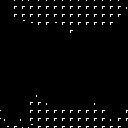
\includegraphics[width=\linewidth]{images/128x128_2.png}
\captionof{figure}{128x128}
\end{Figure}

\begin{Figure}
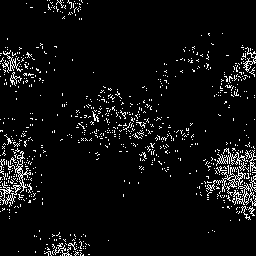
\includegraphics[width=\linewidth]{images/256x256_2.png}
\captionof{figure}{256x256}
\end{Figure}


%column3
\begin{Figure}
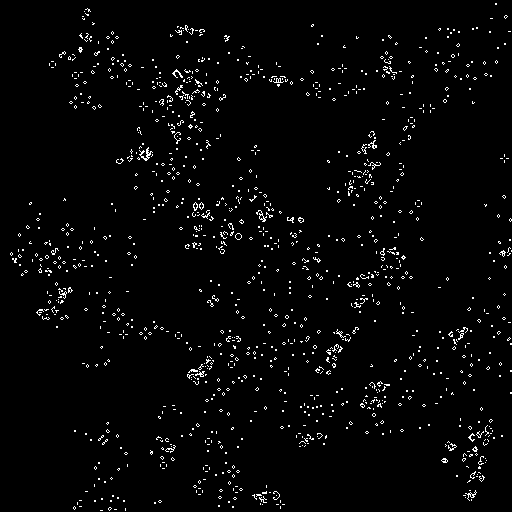
\includegraphics[width=\linewidth]{images/512x512_2.png}
\captionof{figure}{512x512}
\end{Figure}

\end{multicols}

\pagebreak
\section{Critical Analysis}


\bibliographystyle{unsrt}
\bibliography{}
\end{document}